\chapter{Literature Review}
	\section{Brief Table of books}
	\begin{table}[H]
		\begin{tabular}{lllll}
			ISBN 			& Name 	& Type  &  &  \\
			N/A  			&ST1PS-18-9A: Probability and Statistics (2018/19)&Module Lectures&  &  \\
			9780030105678  	&Linear Algebra and Its Applications&Book&  &  \\
			9780131687288  	&Digital Image Processing&Book&  &  \\
			9780262035613  	&Deep Learning &Book&  &  \\
			9780128104088  	&Deep Learning for Medical Image Analysis&Book&  &  \\
			9781491962244  	&Hands-on machine learning with scikit-learn and tensorflow&Book&  &  \\
		\end{tabular}
	\end{table}
	\section{Brief Table of papers}
	\begin{itemize}
		\item Ye, H., Hang, J., Chen, X. et al. An intelligent platform for ultrasound diagnosis of thyroid nodules. Sci Rep 10, 13223 (2020). https://doi.org/10.1038/s41598-020-70159-y
		\item Nguyen DT, Pham TD, Batchuluun G, Yoon HS, Park KR. Artificial Intelligence-Based Thyroid Nodule Classification Using Information from Spatial and Frequency Domains. J Clin Med. 2019;8(11):1976. Published 2019 Nov 14. doi:10.3390/jcm8111976
		\item Manivannan T, Ayyappan N. Classification of thyroid nodules using ultrasound images. Bioinformation. 2020;16(2):145-148. Published 2020 Feb 29. doi:10.6026/97320630016145
		\item Nguyen DT, Kang JK, Pham TD, Batchuluun G, Park KR. Ultrasound Image-Based Diagnosis of Malignant Thyroid Nodule Using Artificial Intelligence. Sensors (Basel). 2020;20(7):1822. Published 2020 Mar 25. doi:10.3390/s20071822
		\item Chen J, You H, Li K. A review of thyroid gland segmentation and thyroid nodule segmentation methods for medical ultrasound images. Comput Methods Programs Biomed. 2020 Mar;185:105329. doi: 10.1016/j.cmpb.2020.105329. Epub 2020 Jan 9. PMID: 31955006.
	\end{itemize}
	\section{Analytic Report: Books}
	\subsection{Learning Path Visualised}
	The reader should note that many of the learning nodes for the following diagram already existed in the student's program in parts 1 and 2. The reference here is sorely for pointing out the need for a complete revision over the aforementioned topics and for clarity.
	\begin{figure}[H]
		\iftrue
		\caption{Learning Path}
		\centering
		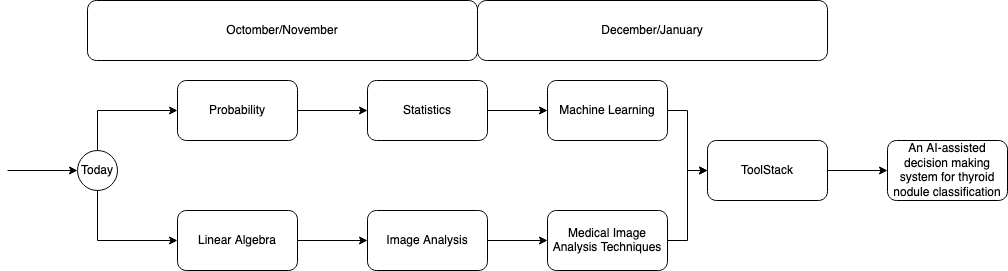
\includegraphics[scale=0.3]{figures/path}
		\fi
	\end{figure}
	\subsection{(Probability/Statistics)ST1PS-18-9A: Probability and Statistics (2018/19)}
	In part 1, my module \textit{Probability and statistics} covers everything essential regarding my statictical background for this project.
	\subsection{(Linear Algebra)Linear Algebra and Its Applications}
	This excellent book will supplement my knowledge of linear algebra, covers almost anything that I will need later in the image analysis part.
	\subsection{(Image Analysis)Digital Image Processing Author(s): Rafael C. Gonzalez, Richard E. Woods + CS3IA16-20-1A: Image Analysis (2020/21)}
	This book, recommended by the lecturer in CS3IA16, will supplement my knowledge in image analysis and basic image transformation algorithms needed for the preprocessing part of the Machine learning service. 
	\subsection{(Machine Learning)Deep Learning Book by Aaron Courville, Ian Goodfellow, and Yoshua Bengio}
	This excellent book is an introduction to Machine learning with Deep Learning techniques, much needed in the AI-analy
	\subsection{(Techniques)Deep Learning for Medical Image Analysis}
	This book has plenty of industry-standard techniques for medical image analysis. It will help me catch up with the latest research methods in this field.
	\subsection{(ToolStack)Hands-On Machine Learning with Scikit-Learn and TensorFlow: }
	This book will teach me the basic AI-toolkit stack, as well as the practical techniques for writing intelligent systems.
	\subsection{Papers}
	Around that time, i will start learning specialized techiques for this domain. The aforementioned papers will be my source of information.	
